\subsection{Game V2}
Game V2 is the game with the even set of rules for the predators and the prey. This game mode should be the mode that provides the closest set of results between the predators and the prey. Unfortunately, the system still seems to provide an advantage to the prey as in every experiment the prey are the agents with the highest fitness. However, unlike in the walled off game and the V1 game, in this game mode, there are times when the predators have a better score than the prey (Figures \ref{fig:v2-pred-better-graphs} and \ref{fig:v2-pred-better-graphs-2}). Unfortunately for the predator, they always get outperformed by the prey. It should be noted that in this case, a core radius of 5 and a perception limit of 30 does make an impact in the initial fitness of the particles, and it is in these cases where the predator fitness is initially higher than the prey fitness.

\begin{figure}
  \centering
  \begin{subfigure}{.7\textwidth}
  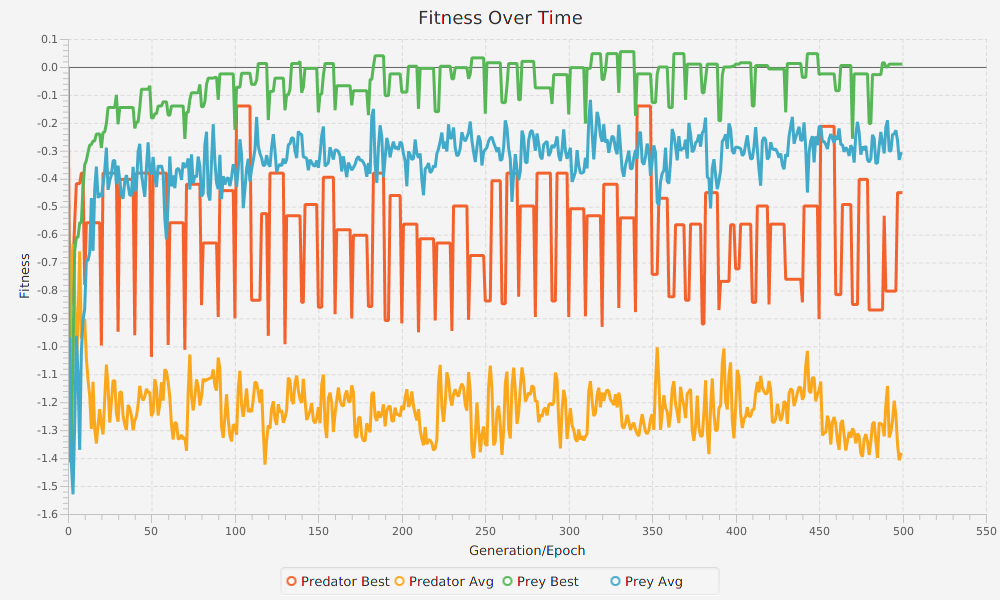
\includegraphics[width=\linewidth]{V2-exp30-Run-2.png}
  \caption{V2 experiment 6 run 3}
  \end{subfigure}
  \begin{subfigure}{.7\textwidth}
  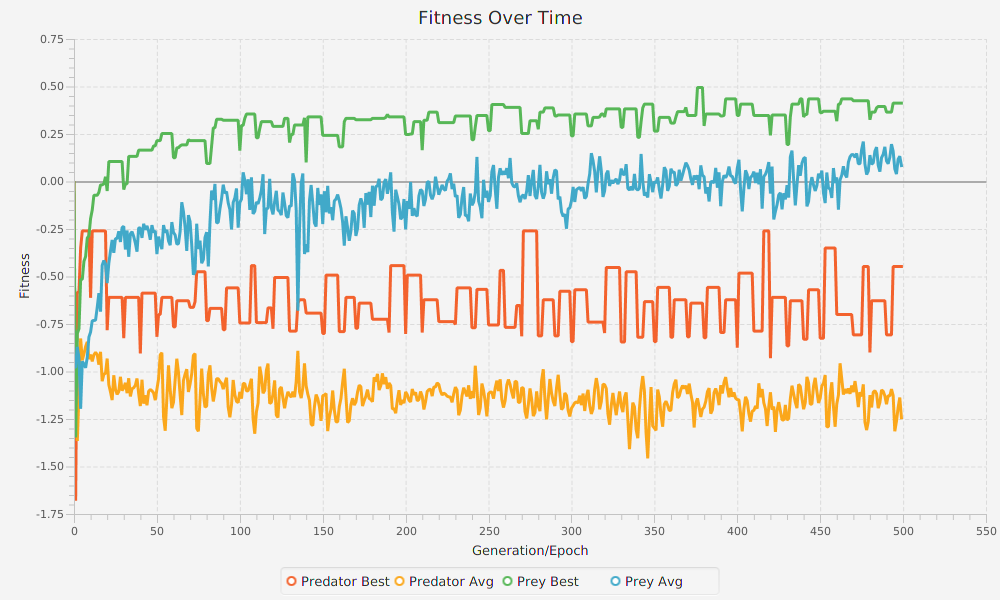
\includegraphics[width=\linewidth]{V2-exp32-Run-4.png}
  \caption{V2 experiment 8 run 5}
  \label{fig:v2-pred-better-graphs}}
  \end{subfigure}
 \end{figure}


\begin{figure}
  \centering
  \begin{subfigure}{.7\textwidth}
  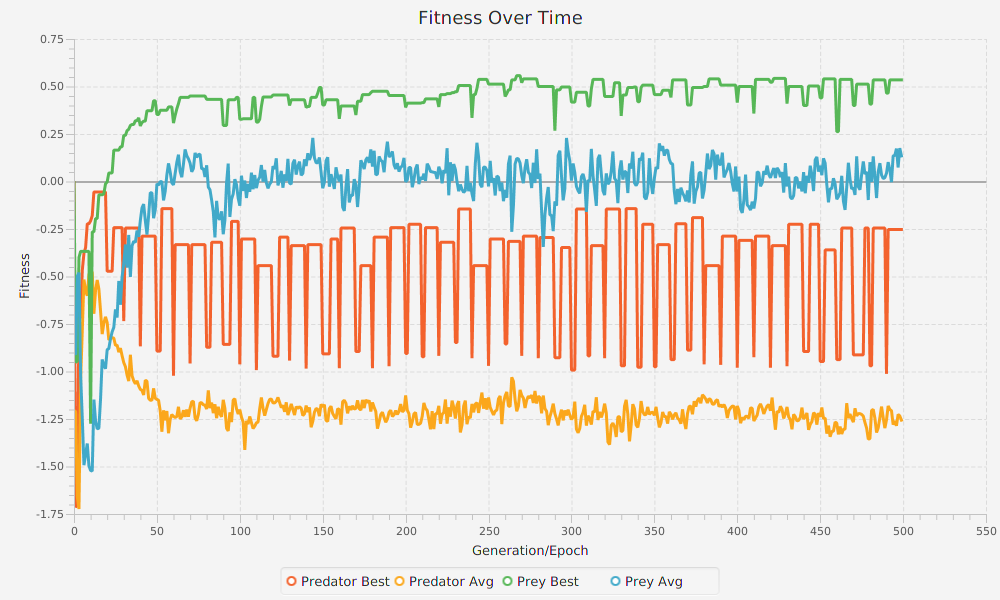
\includegraphics[width=\linewidth]{V2-exp39-Run-0.png}
  \caption{V2 experiment 15 run 1}
  \end{subfigure}
  \begin{subfigure}{.7\textwidth}
  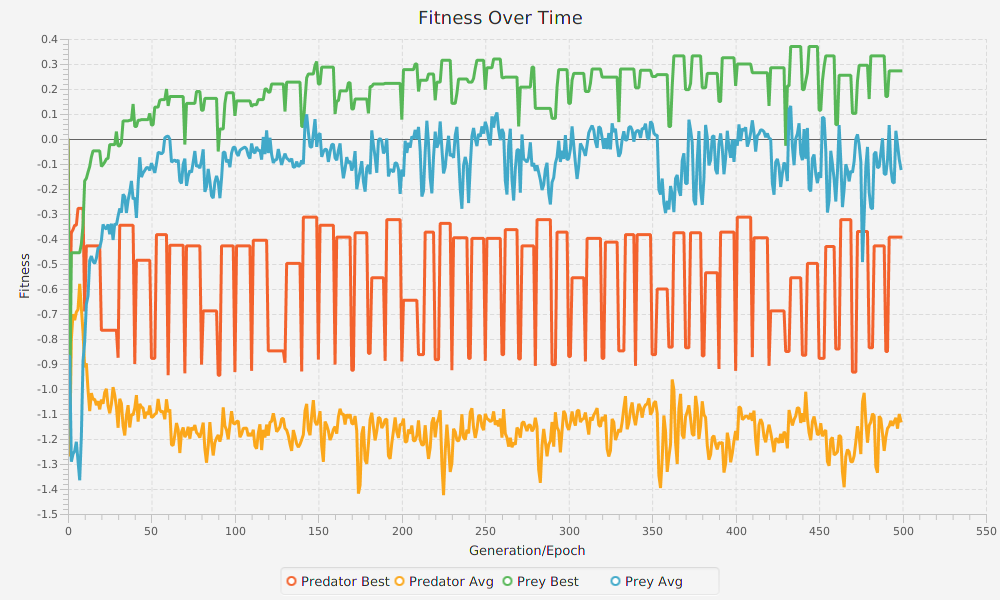
\includegraphics[width=\linewidth]{V2-exp39-Run-3.png}
  \caption{V2 experiment 15 run 4}
  \end{subfigure}
  \caption{Examples of Game V2 fitness over time \label{fig:v2-pred-better-graphs-2}}
\end{figure}

Something of note is that in this game mode, the prey seem to converge as in some games, even when the particles are 67\% charged, the prey experience large drops in fitness when the predators gain a small amount. This can be seen in Figure \ref{fig:v2-prey-large-drop}. 


\begin{figure}
  \centering
  \includegraphics[width=0.7\textwidth]{v2-exp31-Run-2.png}
  \caption{Game V2 experiment 7 run 3: Example of large fitness drop in prey}
  \label{fig:v2-prey-large-drop}
\end{figure}

Observing the games played by the predators in experiment 15 run 1, the predator with one of the highest overall fitnesses can be observed. The games show that the reason this particle received a higher fitness value is because it mostly remained on the board with a couple of captures. As experiment 7 run 3 had the highest fitness value right at the beginning of the run, the movements made by the predator and prey are chaotic with no real structure with the results being similar to game V1 where both the predator and prey just pick a direction to move in and they move in that direction until the game ends (see Figure \ref{fig:v2-exp39-best}). 

\begin{figure}
  \centering
  \includegraphics[width=0.4\textwidth]{v2-exp39-r0-best-Game-370.png}  \includegraphics[width=0.4\textwidth]{v2-exp39-r0-best-Game-388.png}
  \caption{Game V2 experiment 15 Run 1: Example Games}
  \label{fig:v2-exp39-best}
\end{figure}

Taking a look at Game V2 experiment 6 run 3 (as seen in Figure \ref{fig:v2-pred-better-graphs}) it can be seen that the predator with the overall highest fitness appeared later on in the run. This predator adopted a patrolling approach. In most of the runs, the predator tended to move back and forth on the same line and hope that the prey would come that way (see Figure \ref{fig:v2-pred-patrol}). In most cases this did not work and the prey just ran off the board. The major development for the predator is that in most cases, the predator remained on the board.

\begin{figure}
  \centering
  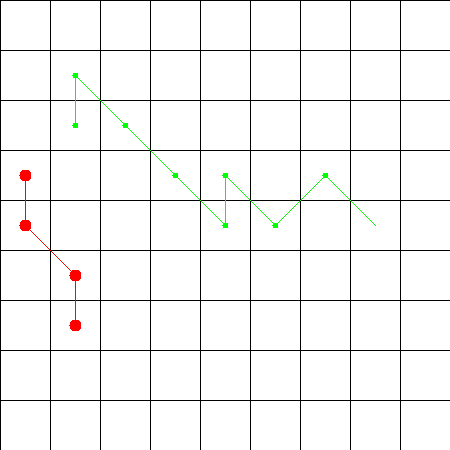
\includegraphics[width=0.4\textwidth]{V2-exp30-r2-Game-152.png}  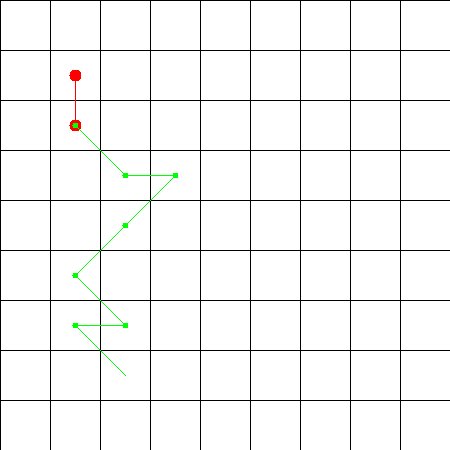
\includegraphics[width=0.4\textwidth]{V2-exp30-r2-Game-362.png}
  \caption{Game V2 experiment 6 run 3: Predator Patrol Example Games}
  \label{fig:v2-pred-patrol}
\end{figure}

As it can be seen in all of the graphs for V2, the prey score has lowered. It is no longer close to 1 as the prey is now penalized for falling off the board. One of the best tactics that the prey evolved is to match the predator's patrol tactic. Using this tactic, the prey just wait for the game to end by patrolling their own area as the predator will never approach the prey anyways. This tactic in can be seen in Figure \ref{fig:v2-prey-patrol}.

\begin{figure}
  \centering
  \begin{subfigure}{\textwidth}
    \centering
  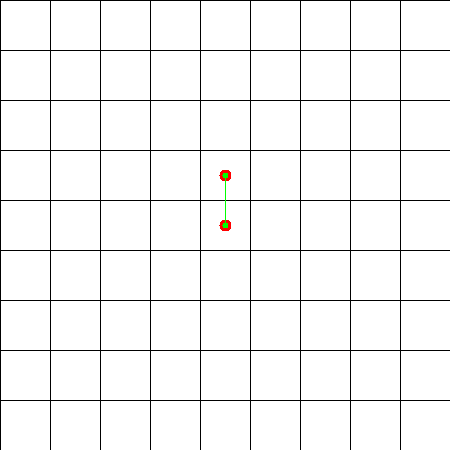
\includegraphics[width=0.4\linewidth]{v2-exp40-py-r4-Game-30.png}  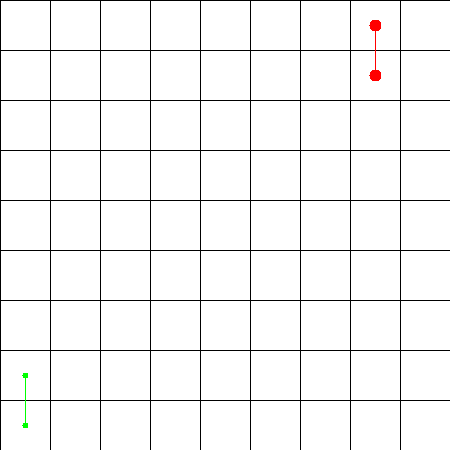
\includegraphics[width=0.4\linewidth]{v2-exp40-py-r4-Game-31.png} 
  \end{subfigure} \\\hfill
  
  \begin{subfigure}{\textwidth}
    \centering
  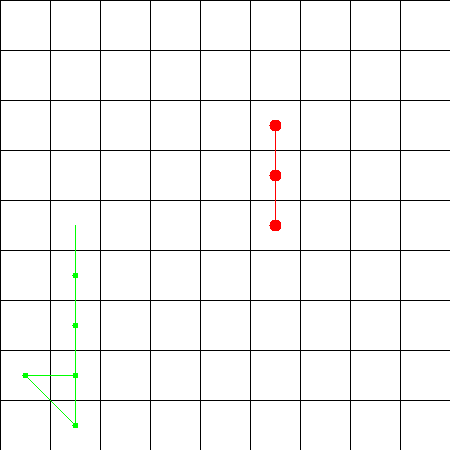
\includegraphics[width=0.4\linewidth]{v2-exp40-py-r4-Game-43.png}
  \end{subfigure}
  \caption{Game V2 Experiment 16 run 5: Prey Patrol Example Games \label{fig:v2-prey-patrol}}
  
\end{figure}


\begin{table}
  \centering
  \begin{tabular}{|c|c|c|c|c|c|c|}
    \hline
    \multirow{2}{*}{Experiment} & \multicolumn{3}{|c|}{Predator} & \multicolumn{3}{|c|}{Prey} \\\cline{2-7}
    & Max & Average & Min & Max & Average & Min\\
    \hline
    1 & -0.300 & -0.384 & -0.488 & 0.576 & 0.373 & 0.237 \\
2 & -0.308 & -0.374 & -0.500 & 0.346 & 0.259 & 0.156 \\
3 & -0.350 & -0.450 & -0.568 & 0.428 & 0.289 & 0.183 \\
4 & -0.315 & -0.392 & -0.515 & 0.471 & 0.252 & 0.044 \\
5 & -0.285 & -0.420 & -0.633 & 0.576 & 0.425 & 0.165 \\
6 & -0.140 & -0.276 & -0.460 & 0.385 & 0.192 & -0.118 \\
7 & -0.055 & -0.409 & -0.563 & 0.507 & 0.319 & 0.122 \\
8 & -0.260 & -0.393 & -0.490 & 0.418 & 0.322 & 0.210 \\
9 & -0.175 & -0.363 & -0.570 & 0.540 & 0.381 & 0.316 \\
10 & -0.160 & -0.322 & -0.468 & 0.519 & 0.407 & 0.298 \\
11 & -0.275 & -0.413 & -0.598 & 0.497 & 0.318 & 0.106 \\
12 & -0.330 & -0.421 & -0.560 & 0.505 & 0.294 & 0.179 \\
13 & -0.130 & -0.373 & -0.713 & 0.531 & 0.378 & 0.148 \\
14 & -0.345 & -0.459 & -0.653 & 0.566 & 0.432 & 0.298 \\
15 & -0.278 & -0.414 & -0.598 & 0.455 & 0.288 & 0.065 \\
16 & -0.305 & -0.443 & -0.520 & 0.510 & 0.410 & 0.315 \\
17 & -0.365 & -0.489 & -0.543 & 0.520 & 0.439 & 0.180 \\
18 & -0.345 & -0.405 & -0.450 & 0.485 & 0.354 & 0.281 \\
19 & -0.173 & -0.361 & -0.533 & 0.486 & 0.264 & -0.020 \\
20 & -0.220 & -0.388 & -0.490 & 0.479 & 0.363 & 0.204 \\
21 & -0.268 & -0.449 & -0.660 & 0.619 & 0.459 & 0.265 \\
22 & -0.280 & -0.413 & -0.738 & 0.446 & 0.293 & 0.144 \\
23 & -0.255 & -0.356 & -0.443 & 0.435 & 0.368 & 0.260 \\
24 & -0.215 & -0.270 & -0.345 & 0.480 & 0.358 & 0.165 \\

    \hline
  \end{tabular}
  \caption{Game V2 Summary}
  \label{tab:v2-summary}
\end{table}

The summary results for game V2 can be seen in Table \ref{tab:v2-summary}. The results are much more varied in this version compared to the results seen in game V1, however in game V2, both the predator and prey achieved better scores on average using the core radius of 5 and perception limit of 30 parameter set. This seems to suggest that allowing the particles to converge closer together before repelling is more beneficial than expanding the search space.
